\documentclass{beamer}
\title{Foroverkoblet reguleringsstruktur}
\author{Fred-Olav}
\begin{document}
\maketitle

%``Feedforward'' is a rather under-used control strategy capable of managing a great many types of process problems.  It is based on the principle of \textit{preemptive load counter-action:} that if all significant loads on a process variable are monitored, and their effects on that process variable are well-understood, a control system programmed to take appropriate action based on load changes will shield the process variable from any ill effect.  That is to say, the feedforward control system uses data from load sensors to predict when an upset is about to occur, then \textit{feeds that information forward to the final control element} to counteract the load change before it has an opportunity to affect the process variable.  Feedback control systems are \textit{reactive}, taking action after to changes in the process variable occur.  Feedforward control systems are \textit{proactive}, taking action before changes to the process variable can occur.
%
%This photograph shows a kind of feedforward strategy employed by human operators running a \textit{retort}: a steam-powered machine used to pressure-treat wooden beams at a milled lumber operation.  The sign taped to this control panel reminds the operator to warn the maintenance department of an impending steam usage:
\begin{frame}
	\frametitle{Fremovermelding}

	
$$\includegraphics[width=15cm]{cont86.eps}$$

\end{frame}

%
%
%The story behind this sign is that a sudden demand in retort steam causes the entire facility's steam supply pressure to sag if it happens at a time when the boiler is idling.  Since the boiler's pressure control system can only react to deviations in steam pressure from setpoint, the boiler pressure controller will not take any action to compensate for sudden demand until \textit{after} it sees the steam pressure fall, at which point it may be too late to fully recover.  If operators give the maintenance personnel advance notice of the steam demand, though, the boiler may be fired up for extra steam capacity and thus will be prepared for the extra demand when it comes.  The upset avoided here is abnormally low steam header pressure, with the predictive load being the retort operator's planned usage of steam.  Crude as this solution might be, it illustrates the fundamental concept of feedforward control: information about a load change is ``fed forward'' to the final control element to preemptively stabilize the process variable.
%
%\vskip 10pt
%
%As the following section explains, perfect feedforward control action is nearly impossible to achieve.  However, even imperfect feedforward action is often far better than none at all, and so this control strategy is quite valuable in process control applications challenged by frequent and/or large variations in load.
%
%
%
%
%
%\filbreak
%\subsection{Load Compensation}
%
%\textit{Feedback} control works on the principle of information from the outlet of a process being ``fed back'' to the input of that process for corrective action.  A block diagram of feedback control looks like a loop:  \index{Feedback control system}
\begin{frame}
	\frametitle{Tilbakekoblet reguleringssystem}

	
$$\includegraphics[width=8cm]{cont05.eps}$$

\end{frame}


%
%\filbreak
%
%The reason any control system is necessary at all\footnote{This statement is true only for self-regulating processes.  Integrating and ``runaway'' processes require control systems to achieve stability even in the complete absence of any loads.  However, since self-regulation typifies the vast majority of industrial processes, we may conclude that the fundamental purpose of most control systems is to counteract the effects of loads.} to maintain a process variable at some stable value is the existence of something called a \textit{load}.  A ``load'' is a variable influencing a process that is not itself under direct control, and may be represented in the block diagram as an arrow entering the process, but not within the control loop:  \index{Load, process}  \index{Process load}
\begin{frame}
	\frametitle{Tilbakekoblet reguleringssystem med forstyrrelser}

	
$$\includegraphics[width=8cm]{cont26.eps}$$

\end{frame}


%
%For example, consider the problem of controlling the speed of an automobile.  In this scenario, vehicle speed is the process variable being measured and controlled, while the final control device is the accelerator pedal controlling engine power output.  If it were not for the existence of hills and valleys, head-winds and tail-winds, air temperature changes, road surface variations, and a host of other ``load'' variables affecting car speed, maintaining a constant speed would be as simple as holding the accelerator pedal at a constant position.
%
%However, the presence of these ``load'' variables makes necessitates a human driver (or a \textit{cruise control} system) continually adjusting engine power to maintain constant speed.  Using the car's measured speed as feedback, the driver (or cruise control) adjusts the accelerator pedal position as necessary based on whether or not the car's speed matches the desired ``setpoint'' value.
%
%An inherent weakness of any feedback control system is that it can never be \textit{proactive}.  The best any feedback control system can ever do is \textit{react} to detected disturbances in the process variable.  This makes deviations from setpoint inevitable, even if only for short periods of time.  In the context of our automobile cruise control system, this means the car can never maintain a \textit{perfectly} constant speed in the face of loads because the control system does not have the ability to anticipate loads (e.g. hills, wind gusts, changes in air temperature, changes in road surface, etc.).  At best, all the feedback cruise control system can do is react to changes in speed it senses \textit{after} some load has disturbed it.
%
%\vskip 10pt
%
%\textit{Feedforward} control addresses this weakness by taking a fundamentally different approach, basing final control decisions on the states of load variables rather than the process variable.  In other words, a feedforward control system monitors the factor(s) influencing a process and decides how to compensate \textit{ahead of time} before the process variable deviates from setpoint.  If all loads are accurately measured, and the control algorithm realistic enough to predict process response for these known load values, the process variable (ideally) need not be measured at all:  \index{Feedforward control strategy}
\begin{frame}
	\frametitle{Tilbakekoblet reguleringssystem som gir forovermelding om forstyrrelser}

	$$\includegraphics[width=8cm]{cont27.eps}$$
	

\end{frame}


%
%As was the case with cascade control, feedforward control also has an analogue in workplace management.  If you consider a supervisor to be the ``controller'' of a work group (issuing orders to his or her subordinates to accomplish important tasks), a feedforward system would be when someone informs the supervisor of an important change that will soon impact the work group.  By having this information ``fed forward'' to the supervisor, the supervisor may then take \textit{preemptive} measures to better manage this change before its effects are fully felt.  If this predictive information is accurate, and the supervisor's response appropriate, any negative impacts of the change will be minimized to the point where no reactive steps will be needed.  Stated differently, good feedforward control action translates what would otherwise be a crisis into an insignificant event.
%
%Returning to the cruise control application, a purely feedforward automobile cruise control system would be interfaced with topographical maps, real-time weather monitors, and road surface sensors to decide how much engine power was necessary at any given time to attain the desired speed\footnote{The load variables I keep mentioning that influence a car's speed constitute an incomplete list at best.  Many other variables come into play, such as fuel quality, engine tuning, and tire pressure, just to name a few.  In order for a purely feedforward (i.e. no feedback monitoring of the process variable) control system to work, \textit{every single load variable} must be accurately monitored and factored into the system's output signal.  This is impractical or impossible for a great many applications, which is why we usually find feedforward control used in conjunction with feedback control, rather than feedforward control used alone.}.  Assuming all relevant load variables are accounted for, the cruise control would be able to maintain constant speed regardless of conditions, and without the need to even monitor the car's speed.
%
%This is the promise of feedforward control: a method of controlling a process variable so perfect in its predictive power that it eliminates the need to even measure that process variable.  If you are skeptical of this feedforward principle and its ability to control a process variable without even measuring it, this is a good thing -- you are thinking critically!  In practice, it is nearly impossible to accurately account for \textit{all} loads influencing a process and to both anticipate and counter-act their combined effects, and so \textit{pure} feedforward control systems are rare\footnote{In fact, the only pure feedforward control strategies I have ever seen have been in cases where the process variable was nearly impossible to measure and could only be inferred from other variables.}.  Instead, the feedforward principle finds use as a supplement to normal feedback control.  To understand feedforward control better, however, we will consider its pure application before exploring how it may be combined with feedback control.
%
%\vskip 10pt
%
%\filbreak
%
%First, let us consider a liquid level control system on an open tank, where three different fluid ingredients (shown in the following P\&ID simply as A, B, and C) are mixed to produce a final product.  A level transmitter (LT) measures liquid level, while a level controller (LC) compares this level to a setpoint value, and outputs a signal calling for a certain amount of discharge flow.  A cascaded (slave) flow controller (FC) senses outgoing flow via a flow transmitter (FT) and works to maintain whatever rate of flow is ``asked'' for by the level controller:
%
\begin{frame}
	\frametitle{Kaskadekoblet reguleringssystem}

	
$$\includegraphics[width=8cm]{cont28.eps}$$

\end{frame}


%The level control system acts to keep liquid level constant in the vessel, ensuring adequate mixing of the three ingredients\footnote{If the liquid level drops too low, there will be insufficient \textit{retention time} in the vessel for the fluids to mix before they exit the product line at the bottom.}.  Being a feedback level control system, it adjusts the discharge flow rate in response to measured changes in liquid level.  Like all feedback control systems, this one is \textit{reactive} in nature: it can only take corrective action \textit{after} a deviation between process variable (level) and setpoint is detected.  As a result, temporary deviations from setpoint are guaranteed to occur with this control system every time the combined flow rate of the three ingredients increases or decreases.  \index{Retention time}
%
%Let us now change the control system strategy from feedback to feedforward.  It is clear what the loads are in this process: the three ingredient flows entering the vessel.  If we measure and sum these three flow rates\footnote{The device or computer function performing the summation is shown in the P\&ID as a bubble with ``FY'' as the label.  The letter ``F'' denotes \textit{Flow}, while the letter ``Y'' denotes a signal relay or transducer.}, then use the total incoming flow signal as a setpoint for the discharge flow controller, the outlet flow should (ideally) match the inlet flow, resulting in a constant liquid level.  Being a purely feedforward control system, there is no level transmitter (LT) any more, just flow transmitters measuring the three loads:
\begin{frame}
	\frametitle{Foroverkoblet reguleringssystem uten tilbakekobling}

	
$$\includegraphics[width=8cm]{cont29.eps}$$

\end{frame}


%
%If all flow transmitter calibrations are perfect, the summing of flow rates flawless, and the flow controller's tuning robust, this level control system should control liquid level in the vessel by proactive effort (``thinking ahead'') rather than reactive effort (``after the fact'').  Any change in the flow rate of ingredients A, B, and/or C is quickly matched by an equal adjustment to the discharge flow rate.  So long as total volumetric flow out of the vessel is held equal to total volumetric flow into the vessel, the liquid level inside the vessel \textit{cannot} change\footnote{Incidentally, this is a good example of an \textit{integrating} mass-balance process, where the rate of process variable change over time is proportional to the imbalance of flow rates in and out of the process.  Stated another way, total accumulated (or lost) mass in a mass-balance system such as this is the time-integral of the difference between incoming and outgoing mass flow rates: $\Delta m = \int_0^T (W_{in} - W_{out}) \> dt$.}.
%
%If this feedforward strategy reminds you of ratio control, you are thinking correctly: the ingredient flow sum signal is the \textit{wild variable}, and the discharge flow signal is the \textit{captive variable}.  The flow controller simply maintains the discharge flow rate at a 1:1 ratio with the (total) ingredient flow rate.  In fact, pure feedforward control is a variation of 1:1 ratio control, except that the real process variable (tank level) is neither the wild (total incoming flow) nor the captive variable (discharge flow) in the process.
%
%\vskip 10pt
%
%An interesting property of feedforward and ratio control systems alike is that they cannot generate oscillations as is the case with an over-tuned (excessive gain) feedback system.  Since a feedforward system does not monitor the effects of its actions, it cannot react to something it did to the process, which is the root cause of feedback oscillation.  While it is entirely possible for a feedforward control system to be configured with too much gain, the effect of this will be \textit{overcompensation} for a load change rather than oscillation.  In the case of the mixing tank feedforward level control process, improper instrument scaling and/or offsets will merely cause the discharge and inlet flows to mis-match, resulting in a liquid level that either continues to increase or decrease over time (``integrate'').  However, no amount of mis-adjustment can cause this feedforward system to produce \textit{oscillations} in the liquid level.
%
%In reality, this pure feedforward control system is impractical even if all instrument calibrations and control calculations are perfect.  There are still loads unaccounted for: evaporation of liquid from the vessel, for example, or the occasional pipe fitting leak.  Furthermore, since the control system has no ``knowledge'' of the actual liquid level, it cannot make adjustments to that level.  If an operator, for instance, desired to decrease the liquid level in order to reduce the residence time (also known as ``retention time'')\footnote{\textit{Residence time} or \textit{Retention time} is the average amount of time each liquid molecule spends inside the vessel.  It is an important variable in chemical reaction processes, where adequate time must be given to the reactant molecules in order to ensure a complete reaction.  It is also important for non-reactive mixing processes such as paint and food manufacturing, to ensure the ingredients are thoroughly mixed together and not stratified.  For any given flow rate through a vessel, the residence time is directly proportional to the volume of liquid contained in that vessel: double the captive volume, and you double the residence time.  For any given captive volume, the residence time is inversely proportional to the flow rate through the vessel: double the flow rate through the vessel, and you halve the residence time.  In some mixing systems where residence time is critical to the thorough mixing of liquids, vessel level control may be coupled to measured flow rate, such that an increase in flow rate results in an increased level setpoint, thus maintaining a constant residence time despite changes in production rate.}, he or she would have to manually drain liquid out of the vessel, or temporarily place the discharge flow controller in ``manual'' mode and increase the flow there (then place back into ``cascade'' mode where it follows the remote setpoint signal again).  The advantage of proactive control and minimum deviation from setpoint over time comes at a fairly high price of impracticality and inconvenience.  \index{Retention time}  \index{Residence time, see Retention time}
%
%\filbreak
%
%For these reasons, feedforward control is most often found in conjunction with feedback control.  To show how this would work in the liquid level control system, we will incorporate a level transmitter and level controller back into the system, the output of that level controller being summed with the feedforward flow signal (by the LY summing relay) before going to the cascaded setpoint input of the discharge flow controller:
\begin{frame}
	\frametitle{Foroverkoblet reguleringssystem med tilbakekobling}

	
$$\includegraphics[width=8cm]{cont30.eps}$$

\end{frame}


%
%This hybrid control strategy is sometimes called \textit{feedforward with trim}.  In this context, ``trim'' refers to the level controller's (LC) output signal contributing to the discharge flow setpoint, helping to compensate for any unaccounted loads (evaporation, leaks) and provide for level setpoint changes.  This ``trim'' signal should do very little of the control work in this system, the bulk of the liquid level stability coming from the feedforward signals provided by the incoming flow transmitters.  \index{Feedforward with trim}  \index{Trim, in a feedforward control system}
%
%%\filbreak
%
%% ADD: elaborate on feedforward with trim versus ratio with trim.
%
%%Recall how pure feedforward control in its simplest form (having no feedback) was likened to a ratio control system with a fixed 1:1 ratio.  With the addition of feedback (trim) to feedforward, we see something that is truly different from what ratio control looked like with the addition of feedback.  In a ratio control system having feedback, the feedback altered the ratio between wild and captive variables.  In a feedforward control system, the feedback merely \textit{offsets} the wild and captive variables.  Using functional diagrams to illustrate:
%
%%$$\includegraphics{.eps}$$
%
%\filbreak
%
%A very similar control strategy commonly used on large steam boilers for the precise control of steam drum water level goes by the name of \textit{three-element feedwater control}.  The following illustration shows an example of this control strategy implemented with pneumatic (3-15 PSI signal) instruments:  \index{Three-element boiler feedwater control}  \index{3-element boiler feedwater control}  \index{Three-element boiler feedwater control}
\begin{frame}
	\frametitle{Tre elements reguleringssystem}

	
$$\includegraphics[width=8cm]{cont31.eps}$$

\end{frame}


%
%Such a control system is called ``three-element'' because it makes use of three process measurements:
%
%\begin{itemize}
%\item Feedwater flow rate
%\item Steam drum water level
%\item Steam flow rate
%\end{itemize}
%
%Feedwater flow is controlled by a dedicated flow controller (FIC), receiving a remote setpoint signal from a summing relay (LY).  The summer receives two inputs: a steam flow signal and the output signal (trim) from the level controller (LIC).  The feedforward portion of this system (steam flow feeding forward to water flow) is intended to match the mass flow rates of water into the boiler with steam flow out of the boiler.  If steam demand suddenly increases, this feedforward portion of the system immediately calls for a matching increase in water flow into the boiler, since every molecule of steam exiting the boiler must come from one molecule of water entering the boiler.  The level controller and transmitter act as a feedback control loop, supplementing the feedforward signal to the cascaded water flow controller to make up for (``trim'') any shortcomings of the feedforward loop.
%
%\vskip 10pt
%
%A three-element boiler feedwater control system is a good example of a feedforward strategy designed to ensure \textit{mass balance}, defined as a state of equality between all incoming mass flow rates and all outgoing mass flow rates.  The steam flow transmitter measures outgoing mass flow, its signal being used to adjust incoming water mass rate.  Since mass cannot be created or destroyed (the Law of Mass Conservation), every unit of steam mass leaving the boiler must be accounted for as an equivalent unit of water mass entering the boiler.  If the control system perfectly balances these mass flow rates, water level inside the boiler \textit{cannot} change.  \index{Mass balance}  \index{Conservation of Mass} 
%
%In processes where the process variable is affected by energy flow rates rather than mass, the balance maintained by a feedforward control system will be \textit{energy balance} rather than mass balance.  Like mass, energy cannot be created or destroyed (the Law of Energy Conservation), but must be accounted for.  A feedforward control system monitoring all incoming energy flows into a process and adjusting the outgoing energy flow rate (or vice-versa) will ensure no energy is depleted from or accumulated within the process, thus ensuring the stability of the processes' internal energy state.   \index{Energy balance}  \index{Conservation of Energy}
%
%\filbreak
%
%An example of energy-balance feedforward control appears in this heat exchanger temperature control system:
\begin{frame}
	\frametitle{Foroverkobling med energibalanse}

	
$$\includegraphics[width=8cm]{cont69.eps}$$

\end{frame}


%
%The two transmitters on the incoming (cold oil) line measure oil temperature and oil flow rate, respectively.  The first ``summing'' function subtracts the incoming oil temperature from the setpoint (desired) temperature, and then the difference of these two temperatures is then multiplied by the flow rate signal to produce a signal representing the \textit{energy demand}\footnote{Energy demand is an example of what is called an \textit{inferred variable}: a physical quantity that we cannot measure directly but instead calculate from measurements made of other variables.} of the incoming oil (i.e. how much energy will be required to elevate the oil flow's temperature to setpoint).  The ``energy demand'' signal is summed with the temperature controller's output signal to set the steam valve position (adding energy to the process).  \index{Inferred variable}
%
%There do exist other loads in this process, such as ambient air temperature and chemical composition of the oil, but these variables are generally less influential on discharge temperature than feed temperature and flow rate.  This illustrates a practical facet of feedforward control: although there may be a great many loads affecting our process variable, we must generally limit our application of feedforward to only the most dominant loads in order to limit control system cost.  Simply put, we usually cannot justify the expense and complexity of a feedforward control system compensating for \textit{every single load} in a system.
%
%
%
%
%\filbreak
%\subsection{Proportioning feedforward action}
%
%Feedforward control works by directly modulating the manipulated variable in a control system according to changes sensed in the load(s).  In order for feedforward to function optimally, it must adjust the manipulated variable in a manner that is proportionate to the need: no more, and no less.  At this juncture it is appropriate to ask the question, ``how do we know the amount of feedforward action that will be adequate for a process, and how do we adjust it if it is too much or too little?''
%
%In processes where the feedforward control strategy attempts to achieve direct mass- or energy-balance, the question of adequate feedforward action is answered in the mathematics of measuring the incoming and outgoing flows.  Consider the following mass-balance level control system where the combined sum of three inlet flows is routed to the setpoint of the exit flow control loop.  In this diagram, the portions of the control strategy implemented as function blocks (algorithms in software) appear inside a yellow-colored bounded area, while all real physical instruments appear outside the yellow area:
\begin{frame}
	\frametitle{}

	
$$\includegraphics[width=8cm]{cont79.eps}$$

\end{frame}


%
%If all flowmeters are calibrated in pounds per minute, then the feedforward signal will likewise be scaled in pounds per minute, and so will the setpoint be for flow control loop.  In a digital control system, it is quite customary to scale each and every analog input signal with some real ``engineering unit'' of measurement, so that the signal will be treated as a physical quantity throughout as opposed to being treated as some anonymous percentage value.  Not only is this consistent scaling a standard feature in digital control systems, but it also helps the implementation of this feedforward control strategy, because we desire the out-going mass flow rate to precisely match the (total) in-coming flow rate.  So long as all flowmeters and their associated scaling factors are accurate, the feedforward control's action \textit{must} be exactly right: an increase of +5 pounds per minute in incoming flow rate will prompt an immediate increase of +5 pounds per minute in outgoing flow rate, simply by virtue of all these measured flows having been scaled in the same unit of measurement.
%
%\vskip 10pt
%
%\filbreak
%
%The situation is not as simple in systems where the feedforward control is not precisely balancing mass-flow or energy rates.  By contrast, let us examine the following pH neutralization system equipped with feedforward control action.  Here, the incoming liquid is alkaline (pH greater than 7), and the control system's job is to mix just enough acid reagent to ``neutralize'' the solution (bring the pH value down to 7):
\begin{frame}
	\frametitle{}

	
$$\includegraphics[width=8cm]{cont80.eps}$$

\end{frame}


%
%Controlling the pH (acidity/alkalinity) of a liquid solution is challenging for many reasons, not the least of which being the need to have adequate mixing time for the reagent to react with the influent.  This mixing time translates to \textit{dead time} in the feedback control system.  If the influent's pH suddenly changes for any reason, the feedback control system will be slow to alter the reagent flow rate due to this dead time, causing long-lasting deviations from setpoint.  The goal of the feedforward signal (from the influent pH transmitter to the summer) is to preemptively adjust reagent flow rate according to how alkaline the incoming flow is, countering any sudden changes in influent pH so the feedback control system doesn't have to take (delayed) action.
%
%Once again, it is appropriate to ask the question, ``how do we know the amount of feedforward action that will be adequate for this process, and how do we adjust it if it is too much or too little?''  It would be blind luck if the system happened to work perfectly as shown, with the influent pH transmitter's signal going straight to the summing function to be added to the pH controller's output signal.  Certainly, an increase in influent pH would cause more acid to be added to the mix thanks to feedforward action, but it would likely add either too much or too little acid than it should.  The scale of the influent pH transmitter does not match the scale of the signal sent to the control valve, and so we do not have a neat ``pound-for-pound'' balance of mass flow as we did in the case of the level control system.  
%
%A neat solution to this problem is to add another function block to the feedforward portion of the control system.  This block takes the influent pH transmitter signal and skews it using multiplication and addition, using the familiar linear equation $y = mx + b$ (where $y$ is the output signal of the function and $x$ is the input signal; $m$ and $b$ being constants).  This function block is typically called a \textit{gain and bias} block:  \index{Gain and bias function block}
\begin{frame}
	\frametitle{}

	
$$\includegraphics[width=8cm]{cont81.eps}$$

\end{frame}


%
%The gain adjustment ($m$) in this function block serves to amplify or attenuate the feedforward signal's magnitude, while the bias adjustment ($b$) offsets it.  
%
%\filbreak
%
%Determining practical values for these ``feedforward tuning constants'' is relatively easy.  First, disable feedback control\footnote{Most control systems' feedforward function blocks are designed in such a way that both the feedback and the feedforward signal paths are disabled when the controller is placed into manual mode, in order to give the human operator 100\% control over the final element (valve) in that mode.  For the purpose of ``tuning'' the feedforward gain/bias function block, one must disable the feedback control \textit{only} so feedforward action is still able to respond to load changes.  If simply switching the feedback controller to manual mode is not an option (which it usually is not), one may achieve the equivalent result by setting the gain value of the feedback controller to zero and ensuring the PID equation is not the ``parallel'' type.  If the PID equation is parallel, you will need to set all three terms (P, I, and D) at their minimum settings.} with the output value at or near 50\%.  Next, introduce load changes to the process while watching the process variable's value after sufficient time has elapsed to see the effects of those load changes.  Increase or decrease the gain value until step-changes in load cease to yield significant changes in the process variable.  The following trends show what too much and too little feedforward gain would look like in this pH control system:
\begin{frame}
	\frametitle{}

	
$$\includegraphics[width=8cm]{cont82.eps}$$

\end{frame}


%
%If the gain is properly set in the gain/bias function block, these load changes should have minimal effect on the process variable.  Step-changes in influent pH should have little effect on the process variable after sufficient time has passed for the load change to have fully propagated through the process.
%
%Once a good gain value has been found, change the bias value until the process variable approaches the normal setpoint value\footnote{This is why it was recommended to leave the feedback controller's output at or near 50\%.  The goal is to have the feedforward action adjusted such that the feedback controller's output is ``neutral,'' and has room to swing either direction if needed to provide necessary trim to the process.}.  
%
%\vskip 10pt
%
%\filbreak
%
%Some control systems provide convenient methods of incorporating feedforward action.  The standard FOUNDATION Fieldbus PID function block, for example, has its own dedicated signal input for feedforward, with feedforward gain as an existing parameter.  The following illustration shows Fieldbus function blocks used to implement normal feedback (PID) control, and also PID with feedforward control: \index{FOUNDATION Fieldbus}
\begin{frame}
	\frametitle{}

	
$$\includegraphics[width=8cm]{cont99.eps}$$

\end{frame}


%
%As you can see, all that is required to augment a FOUNDATION Fieldbus control system with feedforward control action is the addition of one more analog input (AI) function block for the load transmitter, and one connecting line between that block and the PID block's ``\texttt{FF\_Val}'' input.
%
%\vskip 10pt
%
%\filbreak
%
%Other control systems require a bit more programming to implement feedforward.  For example, consider the standard ``Factory Configured Option 101'' function block program for basic PID feedback control in a Siemens model 353 panel-mounted loop controller, contrasted against the version necessary for implementing feedforward action:
\begin{frame}
	\frametitle{}

$$\includegraphics[width=8cm]{pid119.eps}$$

\end{frame}


%
%Note the necessary addition of \textit{two} ``math'' function blocks as well as the extra analog input block for receiving the feedforward (load variable) transmitter's signal: MTH1 needed to add the load transmitter's feedforward signal to the controller's output signal, and MTH2 needed to ensure output tracking still works properly between the PID and A/M function blocks when the human operator switches between automatic and manual modes.  The amount of feedforward action is specified by the ``gain'' parameter for input B of \textit{both} math function blocks, which means any adjustment to feedforward action must be manually entered in two different places!
%





\end{document}
